\documentclass{tietreport}

% Import images
\usepackage{graphicx}

% Diagrams, code listings and tables
\usepackage{tikz}
\usetikzlibrary{arrows.meta,positioning,fit}
\usepackage{listings}
\usepackage{xcolor}
\usepackage{array}

\lstset{
  basicstyle=\ttfamily\small,
  frame=single,
  breaklines=true,
  columns=fullflexible,
  keepspaces=true,
  numbers=left,
  numberstyle=\tiny,
  xleftmargin=2em
}

% Bibliography configuration
\usepackage[
  date=year,
  style=alphabetic,
  backend=biber,
  sorting=nty,
  maxnames=5,
  minnames=3,
  maxalphanames=4,
  minalphanames=3,
  backref=true,
  doi=false,
  isbn=false,
  url=false,
  eprint=false
]{biblatex}
\addbibresource{references.bib}

%% ==================================================
%% CUSTOMIZE THESE FIELDS FOR YOUR PROJECT
%% ==================================================

% Course/Lab header
% TODO: confirm the official course title for UCS503P
\TitlePageHeader{%
  UCS503P - Software Engineering Project%
}

% Main project title
\ProjectTitle{%
  API Gateway%
}

% Subtitle or project description
\ProjectSubTitle{%
  A Self-Service Rate-Limiting Layer for Web APIs%
}

% Student information (up to 4 students)
\author{%
  \texttt{1024030753} Sarthak Jagota \\
  \texttt{1024030755} Palak Mahajan \\
  \texttt{1024030758} Aayush Kumar Singh \\
  \texttt{1024030737} Dushyant Choudhary%
}

% Group number, degree, year, program
% TODO: fill in the group number
\TitlePageSubText{%
  Group: \texttt{XXXX} BE Third Year, CSE%
}

% Faculty advisor/guide name
\AdvisorName{%
  Dr. Paramveer Sidhu%
}

% Evaluation period and department info
\TitlePageFooterText{{%
    \large Mid-Semester Evaluation \\[0.2cm]
    \bfseries Computer Science and Engineering
    Department%
  } \\[0.15cm]
  Thapar Institute of Engineering and Technology,
  Patiala%
}

%% ==================================================

\begin{document}

% Generate title page
\maketitle

% Table of contents (auto-generated from chapters)
\tableofcontents

% ===== CHAPTER 1: INTRODUCTION =====

\chapter{Introduction}

\section{Background and Context}

Publishing a small web API has become cheap. Platform-as-a-service hosts,
managed databases and metered third-party services let a single developer
put an API on the internet in minutes. The same pricing model, however,
moves the cost of each request from a fixed monthly server bill to a
metered, per-request charge. An API that receives more traffic than
expected therefore fails in two ways at once: it slows down for everyone,
and it costs more.

HTTP itself has no notion of a per-client budget. A client may send
requests as fast as it can open connections, and the server learns about
the consequences only afterwards. The standard remedy is a
\emph{rate-limiting gateway}: a reverse proxy placed between clients and
the origin that counts each client's requests and rejects the excess with
HTTP~429 \emph{Too Many Requests}~\cite{rfc6585}. Mature products such as
Kong~\cite{kong}, AWS API Gateway~\cite{awsapigw} and Cloudflare provide
this, but they are either operationally heavy to run or commercially
priced. A developer who only wants to protect one API is otherwise left to
build the counting, storage and enforcement logic alone.

This project builds that missing piece: \textbf{API Gateway}, a
lightweight, self-service gateway that a developer can put in front of an
existing API \emph{without modifying the API}. The developer signs up,
registers the API's URL, chooses a request budget and an algorithm, and
receives a gateway URL and an API key. Clients then call the gateway URL
instead of the origin.

The system is deployed and publicly reachable at
\url{https://api-gateway-yp6s.onrender.com/}, and the source code is
maintained at
\url{https://github.com/bytewithpalak/API-Gateway-Project}.

\subsection{Problem Statement}

Without per-client accounting, an HTTP API suffers from four recurring
failure modes:

\begin{itemize}
  \item \textbf{Resource exhaustion.} One misbehaving client, whether a
    buggy retry loop, a scraper or a deliberate abuser, can saturate
    connection pools and worker threads and degrade service for every other
    client.
  \item \textbf{Uncontrolled cost.} When the API is backed by metered
    resources, unbounded request volume becomes unbounded spending,
    discovered only at billing time.
  \item \textbf{No fairness.} A well-behaved client and an abusive one look
    identical to the server, so capacity goes to whoever sends the most.
  \item \textbf{Expensive remedy.} Existing gateways solve the problem but
    are heavyweight or paid.
\end{itemize}

The engineering core of the problem is not the arithmetic of a rate-limiting
algorithm, which is well known, but \emph{correctness under concurrency and
distribution}. When two gateway instances handle simultaneous requests from
the same client, they must never both observe and consume the same
remaining slot. A limiter that is correct on one thread but over-admits
under concurrent load provides no real protection.

\section{Project Objectives}

The objectives below follow the project proposal submitted on
8~August~2026, and each has a measurable success criterion.

\begin{enumerate}
  \item \textbf{Working reverse proxy with enforcement:} forward requests
    from a gateway URL to a registered origin, relay the origin's response
    unchanged, and reject requests over budget with HTTP~429 and a
    \texttt{Retry-After} header~\cite{rfc9110}.
  \item \textbf{Two selectable algorithms:} implement token bucket and
    sliding window as per-API policies, with all counter state held in
    Redis.
  \item \textbf{Enforcement accuracy (primary metric):} for a limit of $N$
    and $M \gg N$ concurrent requests from one client spread over two
    gateway instances, admit a number of requests within $\pm 2\%$ of $N$.
  \item \textbf{Self-service portal:} user signup and login with JWT, API
    registration with a configurable limit, and an analytics dashboard
    showing allowed versus blocked traffic, traffic over time, and a request
    log.
  \item \textbf{Bounded overhead and reliable logging:} keep the latency the
    gateway adds at p95 $\le 50$\,ms, and record at least 99.9\% of
    requests in the PostgreSQL log with the correct outcome.
  \item \textbf{Explicit failure behaviour and safe proxying:} define,
    implement and test what happens when Redis is unreachable, and prevent
    the gateway from being used as an open proxy into private networks.
  \item \textbf{Continuous delivery:} build and test every change in CI
    and deploy the system on free managed infrastructure.
\end{enumerate}

The work was delivered in weekly iterations, starting from a minimal
proxy-plus-limiter in week one, and split across three parallel
workstreams: gateway and rate limiting, persistence and authentication,
and the analytics frontend.

% ===== CHAPTER 2: METHODOLOGY & DESIGN =====

\chapter{Methodology and Design}

\section{System Architecture}

The system is a three-tier web application with an additional in-memory
tier that holds the rate-limit counters. Figure~\ref{fig:architecture}
shows the components and the path of a proxied request.

\begin{figure}[h]
\centering
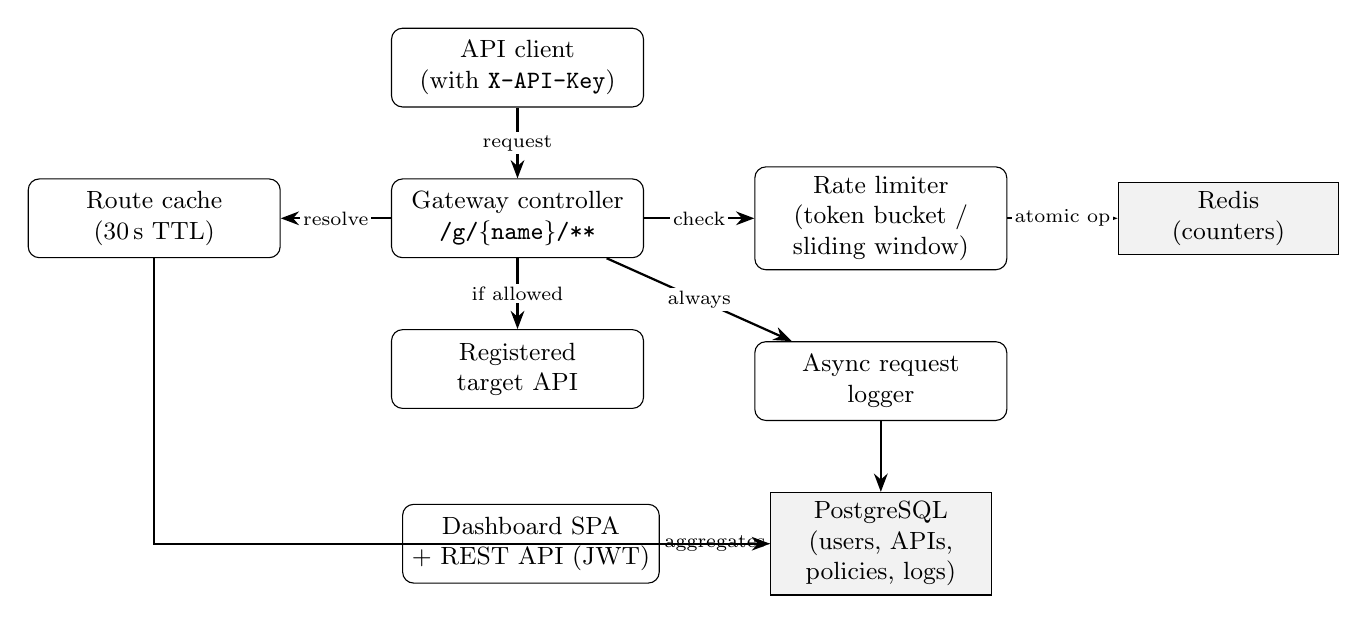
\begin{tikzpicture}[
  node distance=0.9cm and 1.4cm,
  box/.style={draw, rounded corners, align=center, minimum width=3.2cm,
              minimum height=1cm, font=\small},
  store/.style={draw, align=center, minimum width=2.8cm,
                minimum height=0.9cm, font=\small, fill=gray!10},
  arr/.style={-{Stealth}, thick},
  lbl/.style={font=\scriptsize, midway, fill=white, inner sep=1pt}
]
  \node[box] (client) {API client\\(with \texttt{X-API-Key})};
  \node[box, below=of client] (gw) {Gateway controller\\\texttt{/g/\{name\}/**}};
  \node[box, right=of gw] (rl) {Rate limiter\\(token bucket /\\sliding window)};
  \node[store, right=of rl] (redis) {Redis\\(counters)};
  \node[box, below=of gw] (origin) {Registered\\target API};
  \node[box, left=of gw] (cache) {Route cache\\(30\,s TTL)};
  \node[box, below=of rl] (log) {Async request\\logger};
  \node[store, below=of log] (pg) {PostgreSQL\\(users, APIs,\\policies, logs)};
  \node[box, left=of pg] (dash) {Dashboard SPA\\+ REST API (JWT)};

  \draw[arr] (client) -- node[lbl]{request} (gw);
  \draw[arr] (gw) -- node[lbl]{resolve} (cache);
  \draw[arr] (gw) -- node[lbl]{check} (rl);
  \draw[arr] (rl) -- node[lbl]{atomic op} (redis);
  \draw[arr] (gw) -- node[lbl]{if allowed} (origin);
  \draw[arr] (gw) -- node[lbl]{always} (log);
  \draw[arr] (log) -- (pg);
  \draw[arr] (dash) -- node[lbl]{aggregates} (pg);
  \draw[arr] (cache.south) |- (pg.west);
\end{tikzpicture}
\caption{System architecture and request path}
\label{fig:architecture}
\end{figure}

\subsection{High-Level Design}

The design is organised around four components with separate
responsibilities.

\paragraph{Gateway (proxy path).} Every request to
\texttt{/g/\{name\}/...} is handled by a single controller. It resolves the
registered API by its short name, checks the \texttt{X-API-Key} header,
asks the rate limiter for a decision, and then either forwards the request
to the origin or answers with HTTP~429. The remainder of the path after the
API name, the query string, the method, the body and all end-to-end headers
are forwarded unchanged; hop-by-hop headers (such as \texttt{Connection} and
\texttt{Transfer-Encoding}) and the gateway's own API key are stripped.
Redirects from the origin are relayed to the client rather than followed.

\paragraph{Rate limiter and counter store.} All counting state lives in
Redis, so the gateway itself is stateless and any number of instances can
share one budget. Each decision is made by a single atomic operation inside
Redis, which is what prevents two instances from admitting the same slot.

\paragraph{Management API and persistence.} A REST API, protected by JWT
authentication, lets users register APIs, edit their policies, rotate keys
and delete APIs. PostgreSQL stores users, registered APIs, policies and the
request log. The request log is written asynchronously, outside the
client's request path.

\paragraph{Dashboard.} A single-page web application, served by the same
Spring Boot service, reads pre-aggregated statistics over REST and renders
charts, the request log, a test lab and a system health page. Aggregation
happens in the database, so raw logs are never shipped to the browser.

The core request workflow is:

\begin{enumerate}
  \item A developer signs up, logs in, and registers a target API, receiving
    a gateway URL and an API key.
  \item A client sends a request to the gateway URL with the key in the
    \texttt{X-API-Key} header.
  \item The gateway resolves the policy for the API and performs an atomic
    consume-or-reject operation in Redis, keyed by API and client IP.
  \item If allowed, the request is proxied and the origin's response is
    relayed verbatim; otherwise the gateway returns HTTP~429 with
    \texttt{Retry-After}.
  \item In both cases an outcome record is written to PostgreSQL in the
    background.
  \item The dashboard reads aggregated records over REST and renders them.
\end{enumerate}

\subsection{Technical Stack}

\begin{itemize}
  \item \textbf{Framework/Language:} Java~17, Spring Boot~4.1 (Spring Web
    MVC, Spring Data JPA, Spring Security, Bean Validation)~\cite{springboot}.
  \item \textbf{Database:} PostgreSQL~16 for durable data; Redis~7 for
    ephemeral rate-limit counters~\cite{redis}.
  \item \textbf{Libraries:} Bucket4j~8.19 with its Jedis integration for the
    distributed token bucket~\cite{bucket4j}; Jedis~5.2 as the Redis client;
    JJWT~0.12 for JSON Web Tokens~\cite{rfc7519}; BCrypt (via Spring Security)
    for password hashing~\cite{bcrypt}; the JDK \texttt{HttpClient} for
    outbound proxy calls.
  \item \textbf{Frontend:} a dependency-free single-page application in HTML,
    CSS and JavaScript, with charts drawn as inline SVG.
  \item \textbf{Testing:} JUnit~5 and Testcontainers~1.20, which start real
    Redis and PostgreSQL containers for integration tests~\cite{testcontainers}.
  \item \textbf{Tools and deployment:} Maven, Docker and Docker Compose,
    GitHub Actions for CI, Render for hosting (behind Cloudflare), and
    UptimeRobot for availability monitoring.
\end{itemize}

\subsection{Changes from the Proposed Design}

Two parts of the proposed technology stack were replaced during
development. Both were working in early iterations and were changed
deliberately.

\begin{itemize}
  \item \textbf{Spring Cloud Gateway $\rightarrow$ custom proxy controller.}
    Iterations one to three used Spring Cloud Gateway (MVC variant) with
    routes declared in configuration. Once APIs were registered by users at
    runtime and stored in PostgreSQL, every route had to be resolved per
    request from the database, with its own key and policy. The team had
    also hit a filter-ordering problem in week one, where the gateway's
    internal URL-resolution filter ran before our custom filter. A small
    dedicated controller with the JDK \texttt{HttpClient} made the request
    path explicit, removed the version coupling between Spring Boot and the
    Spring Cloud release train, and gave direct control over header
    filtering, timeouts and latency measurement.
  \item \textbf{React + Recharts on Vercel $\rightarrow$ single static page
    served by the backend.} A React dashboard with Recharts was built in an
    earlier iteration. It was later replaced by a single static page served
    by the Spring Boot application, so that the whole system ships as one
    container with one URL and no separate frontend build or hosting. The
    page can still be hosted elsewhere, because the backend's CORS
    configuration allows any origin and authentication uses a bearer header
    rather than cookies.
\end{itemize}

\section{Implementation Details}

\subsection{Module 1: Gateway and Distributed Rate Limiting}

\paragraph{Token bucket.} A bucket of capacity $C$ is refilled at rate
$r = N/W$ tokens per second, where $N$ is the configured limit and $W$ the
window in seconds. Each request consumes one token; a request arriving at an
empty bucket is rejected. This allows controlled bursts up to $C$ while
keeping the long-run average at $r$. The capacity defaults to $N$ and can be
set separately as a burst capacity. The bucket is implemented with Bucket4j's
Redis proxy manager, which uses compare-and-swap updates so that concurrent
consumers from different instances cannot both take the last token. The
policy values are part of the Redis key, so editing a policy starts fresh
buckets rather than reusing ones built with the old numbers. Idle buckets
expire automatically once they would be full again.

\paragraph{Sliding window.} An early version used Bucket4j's interval
refill, but this behaves as a \emph{fixed} window: a client can send $N$
requests at the end of one window and $N$ more at the start of the next,
reaching $2N$ in a short span. It was replaced with a true sliding window
(a ``sliding log''), implemented as one Lua script that Redis executes
atomically (Listing~\ref{lst:sliding}). Each admitted request is stored as a
timestamp in a sorted set; entries older than the window are removed, and a
request is admitted only if fewer than $N$ remain. The script uses Redis's
own clock, so differences between gateway instances' clocks cannot affect
the result. When a request is rejected, the script returns the exact time
until the oldest entry leaves the window, which becomes the
\texttt{Retry-After} value.

\begin{lstlisting}[caption={Atomic sliding-window check in Redis (Lua)},
                   label={lst:sliding}]
local key    = KEYS[1]
local window = tonumber(ARGV[1])
local limit  = tonumber(ARGV[2])
local t      = redis.call('TIME')
local now    = tonumber(t[1]) * 1000 + math.floor(tonumber(t[2]) / 1000)
redis.call('ZREMRANGEBYSCORE', key, 0, now - window)
if redis.call('ZCARD', key) < limit then
  redis.call('ZADD', key, now, ARGV[3])
  redis.call('PEXPIRE', key, window)
  return -1
end
local oldest = redis.call('ZRANGE', key, 0, 0, 'WITHSCORES')
return tonumber(oldest[2]) + window - now
\end{lstlisting}

\paragraph{Retry-After.} For both algorithms the gateway reports the real
time until the next request would succeed, rounded up to whole seconds,
rather than the length of the whole window.

\paragraph{Failure policy when Redis is unreachable.} This is an explicit,
configurable decision. \emph{Fail-open} (the default) admits traffic without
limits, preserving the API's availability; \emph{fail-closed} rejects
traffic, preserving protection. The default is fail-open because a Redis
outage that took every protected API offline would be worse, for most
users, than a short period without limiting. Redis calls use a 500\,ms
socket timeout, and after one failure the limiter skips Redis for five
seconds (a minimal circuit breaker), so an outage does not add a timeout to
every request. The policy can be changed from the dashboard's System page,
which also shows whether Redis is currently up.

\paragraph{Client identity.} Budgets are kept per client IP address. The
production deployment runs behind Cloudflare, where the socket address is a
Cloudflare edge server that changes between requests; this initially spread
one client's requests over many buckets. The gateway can therefore be
configured to read the real client IP from the \texttt{CF-Connecting-IP}
header. The option is off by default, because trusting such a header on a
directly reachable server would let clients choose their own identity.

\paragraph{Route cache.} Looking up the API and policy in PostgreSQL on every
request would add database latency to the proxy path. Routes are cached for
30 seconds; edits made from the dashboard evict the entry immediately on
the instance that handled them and take effect on other instances within
30 seconds.

\subsection{Module 2: Persistence, Authentication and Security}

\paragraph{Data model.} Four entities are stored in PostgreSQL:
\texttt{users} (email and BCrypt hash), \texttt{registered\_apis} (owner,
name, unique short name, target URL, unique API key, active flag),
\texttt{policies} (one per API: algorithm, limit, window, optional burst
capacity) and \texttt{request\_logs} (API, client identity, outcome, HTTP
status, gateway-added latency, timestamp). The request log has a composite
index on \texttt{(api\_id, timestamp)}, which matches every dashboard query.

\paragraph{Authentication.} Users sign up and log in with an email and
password; passwords are hashed with BCrypt and never stored in plain text.
A successful login returns a signed JWT that the dashboard sends as a bearer
token. The API is stateless (no server sessions), and an expired or missing
token returns HTTP~401 so the dashboard can send the user back to the login
page. Every management and dashboard endpoint returns only the caller's own
APIs, and requests for another user's API return 404 rather than 403, so API
identifiers are not revealed.

\paragraph{Proxy-abuse (SSRF) protection.} A gateway that forwards to
arbitrary URLs could be abused to reach internal services or cloud metadata
endpoints~\cite{owaspssrf}. The gateway only forwards to targets registered
by an authenticated owner, and each target URL is validated: it must use
\texttt{http} or \texttt{https}, and \emph{every} address its host resolves
to must be public. Loopback, link-local (including the
\texttt{169.254.169.254} metadata address), private, any-local, multicast
and IPv6 unique-local addresses are refused. The check runs at
registration and again whenever a route is reloaded, so a domain later
pointed at an internal address stops working.

\paragraph{Secrets.} Database credentials, the Redis URL and the JWT signing
key are read from environment variables configured on the hosting platform,
not from the repository. API keys are random UUIDs and can be rotated from
the dashboard; the old key stops working immediately.

\subsection{Module 3: Request Logging and Analytics}

\paragraph{Asynchronous logging.} After each decision the gateway calls an
\texttt{@Async} logging service, so the database write happens on a
separate thread pool and never adds to the client's response time. The
trade-off is that a crash between sending the response and writing the row
loses that row; the log-completeness metric exists to measure this risk.

\paragraph{Gateway-added latency.} For each proxied request the gateway
records its total handling time minus the time spent waiting for the
origin. This isolates the overhead the gateway itself adds, which is the
quantity the latency objective concerns.

\paragraph{Dashboard endpoints.} All aggregation is done in PostgreSQL:
allowed versus blocked counts per API over the last 24 hours, 24 hourly
traffic buckets for the chart, p50 and p95 gateway-added latency (using
\texttt{percentile\_cont}), recent throughput, and a paginated request log
filterable by outcome and API. Page sizes are capped at 100 rows.

\paragraph{Dashboard pages.} The single-page application provides:
an \emph{overview} with totals and a 24-hour traffic chart; \emph{My APIs}
for registering, editing, rotating keys and deleting APIs, with a
ready-to-copy \texttt{curl} example; \emph{Request logs} with filters and
pagination; a \emph{Test lab} that fires a configurable number of concurrent
requests at one of the user's gateway URLs and reports admitted, blocked and
deviation from the limit, plus a simulated side-by-side comparison of the
two algorithms; and a \emph{System} page with Redis health, the fail policy
and latency figures. The layout is responsive and works on phone-width
screens.

\subsection{Module 4: Build, Test and Deployment}

A GitHub Actions workflow runs \texttt{mvn verify} on every push and pull
request, which compiles the application and runs the full integration test
suite against real Redis and PostgreSQL containers. A multi-stage
Dockerfile builds the application with Maven and packages it on a slim
Java~17 runtime image. Docker Compose starts the whole system (application,
PostgreSQL and Redis) locally with one command. In production the container
runs on Render, which redeploys automatically when commits reach the main
branch, and UptimeRobot checks the site periodically, which also keeps the
free-tier instance from sleeping.

% ===== CHAPTER 3: RESULTS & EVALUATION =====

\chapter{Results and Evaluation}

\section{Testing Methodology}

\begin{itemize}
  \item \textbf{Unit Testing:} Rate-limiter behaviour, including the Redis
    failure path, is tested directly against the \texttt{RateLimiter} class,
    without starting the web application. Repository queries are tested in
    isolation for each filter.
  \item \textbf{Integration Testing:} All automated tests run against
    \emph{real} Redis~7 and PostgreSQL~16 instances started by
    Testcontainers, not in-memory substitutes, because the behaviour being
    tested (atomic Redis operations, the async thread pool, PostgreSQL's
    connection pool) differs in ways that matter. The suite runs in CI on
    every push.
  \item \textbf{Concurrency and multi-instance testing:} The accuracy test
    creates two independent rate-limiter instances, each with its own Redis
    connection pool, exactly as two application servers would have. It sends
    400 requests from 32 threads for a single client, alternating between
    the two instances, against a limit of $N = 20$ with a one-hour window
    (so no refill happens during the test), for both algorithms. Earlier, a
    manual test also ran two full gateway processes on ports 8080 and 8081
    against one Redis and alternated requests between them.
  \item \textbf{Performance Testing:} Gateway overhead was benchmarked by
    comparing 20 requests sent directly to an origin (httpbin) with 20 sent
    through the gateway, using persistent connections on both sides. In
    production, every request's gateway-added latency is logged and the p50
    and p95 are shown on the System page.
  \item \textbf{Manual and API testing:} Endpoints were exercised with
    \texttt{curl}, Postman and the browser, including refill behaviour,
    stopping Redis while the gateway was running, and CORS behaviour from a
    browser origin.
  \item \textbf{User Testing:} A structured usability study with external
    developers has not yet been carried out (see Section~\ref{sec:analysis}).
\end{itemize}

\section{Performance Metrics}

Table~\ref{tab:tests} lists the automated test suite, run on
15~October~2026 with Docker and Testcontainers. All eight tests passed.

\begin{table}[h]
\centering
\begin{tabular}{|l|p{6.6cm}|c|}
  \hline
  \textbf{Test} & \textbf{What it verifies} & \textbf{Result} \\
  \hline
  \texttt{tokenBucketIsExact...} & Token bucket, 2 instances, 400 requests,
    $N=20$ & 20 admitted \\
  \hline
  \texttt{slidingWindowIsExact...} & Sliding window, 2 instances, 400
    requests, $N=20$ & 20 admitted \\
  \hline
  \texttt{failOpenAndFailClosed...} & Redis down: open allows, closed
    blocks, breaker answers in $<50$\,ms & Pass \\
  \hline
  \texttt{concurrentAsyncLogging...} & 2000 concurrent async log writes
    reach PostgreSQL & 2000 / 2000 \\
  \hline
  \texttt{filtersByOutcome} & Log filter by outcome & Pass \\
  \hline
  \texttt{filtersByClientIdentity} & Log filter by client & Pass \\
  \hline
  \texttt{filtersByDateRange} & Log filter by date range & Pass \\
  \hline
  \texttt{neverLeaksAcrossApiId} & No rows from another API & Pass \\
  \hline
\end{tabular}
\caption{Automated test suite results (8 tests, 0 failures)}
\label{tab:tests}
\end{table}

Table~\ref{tab:performance} compares the measured results with the targets
set in the proposal.

\begin{table}[h]
\centering
\begin{tabular}{|p{4.2cm}|p{2.6cm}|p{6.2cm}|}
  \hline
  \textbf{Metric} & \textbf{Target} & \textbf{Achieved} \\
  \hline
  Enforcement accuracy, 2 instances, $M = 20N$ & within $\pm 2\%$ of $N$ &
    $20/20$ admitted for both algorithms (0\% deviation) \\
  \hline
  Enforcement accuracy, single instance (week~3) & within $\pm 2\%$ of $N$ &
    $20$ of $200$ admitted, $N = 20$ (0\% deviation) \\
  \hline
  Shared budget across two running gateways (manual) & one shared budget &
    budget shared; both ports returned 429 once it was spent \\
  \hline
  Gateway-added latency & p95 $\le 50$\,ms & $\approx 26.5$\,ms mean over 20
    requests (local benchmark); deployed p95 not yet recorded \\
  \hline
  Log completeness & $\ge 99.9\%$ & $100\%$ (2000 of 2000 concurrent
    writes) \\
  \hline
  Redis failure handling & defined and tested & fail-open and fail-closed
    both verified; breaker responds in under 50\,ms \\
  \hline
  Availability & $\ge 99\%$ & monitored with UptimeRobot; figure for the
    pilot window not yet reported \\
  \hline
\end{tabular}
\caption{Measured results against proposal targets}
\label{tab:performance}
\end{table}

\section{Analysis}
\label{sec:analysis}

\paragraph{Objectives met.} The primary objective, enforcement accuracy
under concurrent load across two instances, was met exactly: both algorithms
admitted precisely $N$ requests out of $20N$, which is better than the
$\pm 2\%$ target. This confirms that performing each decision as one atomic
operation inside Redis (compare-and-swap for the token bucket, a single Lua
script for the sliding window) removes the race condition the project set
out to address. Log completeness was 100\% under 2000 concurrent writes, and
the Redis failure path behaves as configured. Objectives 1, 2, 4 and 6 are
fully implemented, and the system is deployed and publicly reachable.

\paragraph{Partly met.} The local latency benchmark ($\approx 26.5$\,ms
added) is well inside the 50\,ms budget, but it is a mean over 20 requests,
not a p95 on the deployed system. The deployed system now records
gateway-added latency for every request, so the p95 can be reported
directly from the System page after a measurement run. The two-instance
accuracy test runs both limiter instances in one test process against one
real Redis; a run against two deployed instances, with requests counted at
the origin, would make the evidence stronger. CI builds and tests every
change, but linting, container image publishing and a separate staging
environment are not yet part of the pipeline.

\paragraph{Not yet done.} The usability study with 5--10 developers,
measurement of dashboard freshness and sustained throughput per instance
count, and the stretch goal of request replay remain open. The algorithm
comparison in the Test lab is a client-side simulation rather than a live
run of both algorithms under identical load.

\paragraph{Challenges and how they were resolved.}

\begin{itemize}
  \item \textbf{Stale bucket state.} Bucket4j applies a bucket's
    configuration only when the bucket is first created in Redis, so policy
    edits were silently ignored. Including the policy values in the Redis
    key fixed this: an edited policy starts new buckets.
  \item \textbf{Fixed window instead of sliding window.} The first
    ``sliding window'' used interval refill, which allows up to $2N$
    requests around a window boundary. It was replaced with the atomic
    sliding-log Lua script.
  \item \textbf{Wrong client identity behind Cloudflare.} In production,
    one client appeared as many different Cloudflare edge IPs and received
    many budgets. Reading \texttt{CF-Connecting-IP}, behind a configuration
    switch, fixed this without making local deployments spoofable.
  \item \textbf{Misleading latency benchmark.} The first benchmark showed
    the gateway as 760\,ms \emph{faster} than calling the origin directly,
    because each direct \texttt{curl} call paid a fresh TLS handshake while
    the gateway reused a warm connection. Using persistent connections on
    both sides gave the realistic 26.5\,ms figure.
  \item \textbf{Testcontainers and Docker API mismatch.} Recent Docker
    Desktop versions rejected the client bundled with Testcontainers~1.20.
    Pinning the Docker API version in \texttt{docker-java.properties}
    resolved it.
  \item \textbf{Browser-only failures.} Requests that worked in
    \texttt{curl} failed in the browser because of CORS preflight rules and
    the browser's native login pop-up on HTTP~401. The CORS configuration
    was corrected and unauthenticated responses no longer trigger the
    pop-up, which showed that \texttt{curl} tests alone do not cover
    browser clients.
\end{itemize}

% ===== CHAPTER 4: CONCLUSION =====

\chapter{Conclusion}

\section{Summary of Work}

The project delivered API Gateway, a deployed, self-service rate-limiting
reverse proxy that protects an existing API without modifying it. A
developer can sign up, register an API, choose between token bucket and
sliding window, and receive a gateway URL and key; clients over budget
receive HTTP~429 with an accurate \texttt{Retry-After}. Counters live in
Redis and are updated atomically, so the limit holds across gateway
instances. Every request is logged asynchronously to PostgreSQL and
summarised on a responsive dashboard with traffic charts, a filterable
request log, a load-testing lab and a system health page. The system is
protected against SSRF, has an explicit and tested Redis failure policy,
is tested in CI against real Redis and PostgreSQL, and runs as a single
Docker container on Render.

Of the objectives in Section~1.2, the proxy and enforcement, both
algorithms, the primary accuracy metric, the self-service portal, failure
handling and safe proxying, and CI with deployment have been met. The
latency target is met on the local benchmark but still needs a p95
measured on the deployed system.

\section{Key Findings}

\begin{itemize}
  \item \textbf{Finding 1:} Atomicity, not the algorithm, decides
    correctness. With every decision made by a single atomic Redis operation,
    two independent instances admitted exactly $N$ of $20N$ concurrent
    requests for both algorithms.
  \item \textbf{Finding 2:} Library behaviour can quietly change the
    algorithm. Bucket4j's interval refill, used as a ``sliding window'',
    actually behaves as a fixed window, and Bucket4j keeps the configuration
    a bucket was created with. Both were found only by testing the system's
    real behaviour rather than trusting its configuration.
  \item \textbf{Finding 3:} Deployment details affect correctness. Behind a
    CDN, the socket address is not the client, which silently broke
    per-client limits in production until the real client IP was read from
    a trusted header.
  \item \textbf{Finding 4:} Measurement method matters as much as the
    system. Comparing cold and warm connections made the gateway look 760\,ms
    faster than the origin; only a like-for-like benchmark gave a meaningful
    overhead figure.
\end{itemize}

\section{Future Work and Recommendations}

\begin{enumerate}
  \item \textbf{Complete the evaluation:} run a scripted load test against
    two deployed instances and count admitted requests at the origin; report
    deployed p50/p95 overhead, sustained throughput per instance count,
    dashboard freshness and uptime over a fixed pilot window; and carry out
    the usability study with 5--10 developers.
  \item \textbf{Strengthen the pipeline:} add static analysis and linting,
    build and publish the container image in CI, add a staging environment
    before production, and fail the build when p95 overhead exceeds the
    budget.
  \item \textbf{Product features:} request replay from the log, a live
    side-by-side comparison of the two algorithms, client and date filters
    in the log view, and per-API-key (not only per-IP) budgets.
  \item \textbf{Operational hardening:} store the fail policy centrally
    rather than per instance and restrict who may change it, require the JWT
    secret to be set rather than falling back to a development default, and
    move to a durable log pipeline (for example a queue) so that a crash
    cannot drop log rows.
  \item \textbf{Scalability:} use pre-aggregated summary tables for the
    dashboard as log volume grows, and run Redis with replication so the
    counter store is not a single point of failure.
\end{enumerate}

\section{Final Remarks}

The project showed that the hard part of rate limiting is not the formula
but keeping it correct when many requests arrive at once on more than one
server, and when the system runs behind real infrastructure such as a CDN.
Building on mature components (Spring Boot, Redis, Bucket4j, PostgreSQL)
let the team spend its effort on that correctness, on testing it against
real services, and on measuring it honestly. The result is a working,
deployed gateway that a developer can put in front of an API in a few
minutes, and a clear list of the measurements that remain to complete the
evaluation.

% ===== BIBLIOGRAPHY =====

% Print bibliography with heading in TOC
\printbibliography[heading=bibintoc]

\end{document}
